% ============================================================
% Digital Discovery Results — honest structure-based ML benchmark
% Repositioned 2026-06-23 (see HONEST_ML_ASSESSMENT_260622.md). All numbers trace to
% data/final_model_metrics.json, data/structural_rebuild_metrics.json,
% data/dft_benchmark_comparison.csv.
% ============================================================

\section{Results and Discussion}\label{sec:results}

\subsection{Why we target the measured gap: ruling out a circular benchmark}\label{subsec:circularity}

A natural temptation is to regress the singlet--triplet gap
$\Delta E_\text{ST}$ onto a feature set that already contains the $S_1$ and $T_1$
excitation energies. Because $\Delta E_\text{ST} \equiv E_{S_1} - E_{T_1}$ by
definition, such a model reproduces its target to within numerical noise: in our
data the sTDA gap equals $E_{S_1}-E_{T_1}$ with correlation $1.000$ and zero mean
absolute error. A support-vector regressor trained this way reaches an in-sample
cross-validated $R^2 = 0.87$, but this number measures arithmetic, not learning---a
direct subtraction of two input features outperforms the regressor. We therefore
discard the semi-empirical gap as a target and benchmark models on the only
non-trivial quantity: the \emph{experimentally measured} $\Delta E_\text{ST}$.

\subsection{Structure-based models predict experimental gaps with modest, honestly-bounded accuracy}\label{subsec:benchmark}

\begin{figure}[htbp]
  \centering
  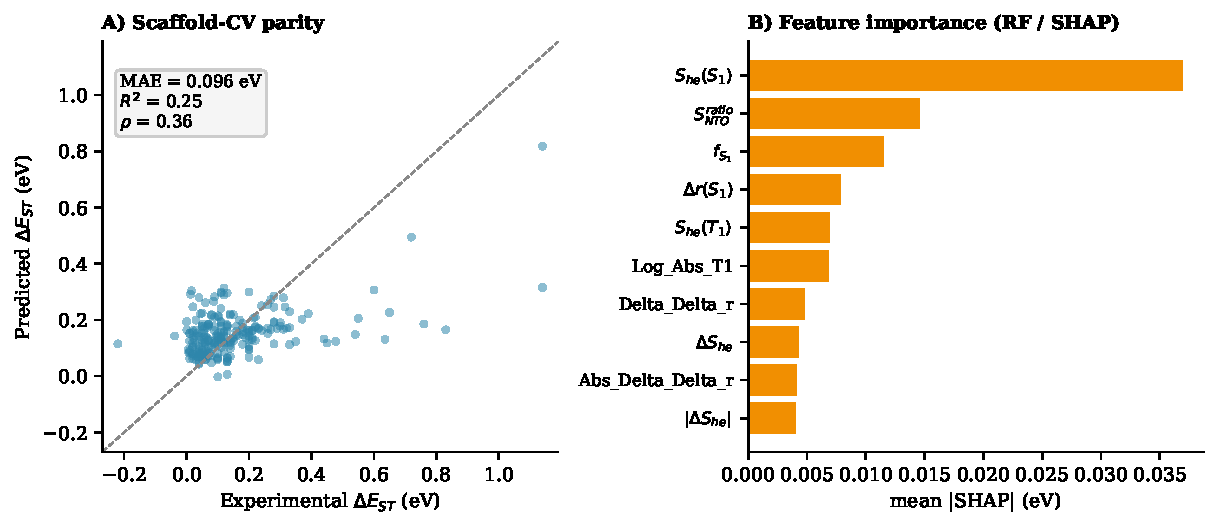
\includegraphics[width=0.95\textwidth]{figures/fig1_model_performance.pdf}
  \caption{Structure-based prediction of experimental $\Delta E_\text{ST}$.
    (A)~Scaffold cross-validated parity for the random forest on NTO
    spatial descriptors (\num{231} molecules, \num{212} Bemis--Murcko scaffolds):
    MAE = \qty{0.096}{\electronvolt}, $R^2 = 0.25$, Spearman $\rho = 0.36$. Models
    built from the 2D structure alone (Morgan, RDKit) perform equivalently
    (\cref{tab:feature_comparison}). The
    model regresses high-gap outliers toward the mean, the expected behaviour
    when the training distribution is dominated by low-gap emitters.
    (B)~SHAP importances: hole--electron overlap $S_\text{he}$, NTO overlap ratio,
    oscillator strength $f_{S_1}$ and charge-transfer distance $\Delta r$ dominate,
    consistent with exchange-integral physics.}
  \label{fig:model_performance}
\end{figure}

We assembled \num{231} donor--acceptor molecules for which an experimental
$\Delta E_\text{ST}$ could be matched to a structure, and evaluated random-forest
regressors under Bemis--Murcko scaffold cross-validation (\num{212} distinct
scaffolds), so that no scaffold appears in both training and test.
Because \qty{92.9}{\percent} of scaffolds are singletons, this split and a random
split produce numerically similar folds---test-set nearest-neighbour Tanimoto to
the training set differs by only \num{0.022}---so the protection is chemical (zero
shared scaffolds per fold, versus \numrange{3}{8} under a random split) rather than
a large change in task difficulty. That the model learns real signal rather than
scaffold-group structure is confirmed by a label-permutation test: the true
scaffold-CV MAE (\qty{0.096}{\electronvolt}) lies far below the null from
\num{1000} target shuffles (mean \qty{0.121}{\electronvolt}, $p = 0.001$;
\cref{SI-tab:scaffold}).
The headline accuracy is also robust to the validation scheme: replacing the singleton
scaffolds with genuine multi-molecule Butina clusters (down to \num{70} groups, largest
\num{38} molecules) leaves the MAE at \qtyrange{0.099}{0.104}{\electronvolt}, between
scaffold-CV (\qty{0.096}{\electronvolt}) and random-CV (\qty{0.106}{\electronvolt})
(\cref{SI-tab:clustercv}).
Three feature sets give statistically indistinguishable performance
(\cref{tab:feature_comparison}). Two are computed from the 2D structure alone, with
no quantum chemistry: Morgan fingerprints (MAE = \qty{0.091}{\electronvolt}) and
RDKit physicochemical descriptors (\qty{0.100}{\electronvolt}). The third, NTO spatial
descriptors, is derived from a semi-empirical sTDA excited-state calculation but
excludes the $S_1$/$T_1$ energy scalars; it reaches MAE = \qty{0.096}{\electronvolt}
(\qty{95}{\percent} CI \numrange{0.082}{0.109}), $R^2 = 0.25$ (CI
\numrange{0.03}{0.45}), Spearman $\rho = 0.36$.
That the structure-only sets match the NTO set is the central methodological point:
the excited-state calculation buys nothing, and adding back the $S_1$/$T_1$ energies
does not help either (\cref{tab:feature_comparison}).
The honest comparator is the mean-value baseline (MAE = \qty{0.107}{\electronvolt}),
over which every model improves by only about \qty{10}{\percent}; the large apparent
gain over the raw sTDA gap (\qty{0.25}{\electronvolt}) reflects that the semi-empirical
gap is badly biased, not that the model is accurate.
The $R^2$ confidence intervals are wide and, for the structure-only sets, include
negative values (RDKit \numrange{-0.11}{0.51}; Morgan \numrange{-0.19}{0.53}): at
\qty{95}{\percent} confidence we cannot exclude that these models are no better than
predicting the mean. The signal is real but weak.

\begin{table}[htbp]
  \centering
  \caption{Prediction of experimental $\Delta E_\text{ST}$ under scaffold
    cross-validation (random forest, \num{231} molecules); $R^2$ with \qty{95}{\percent}
    bootstrap CI. The 2D-structure-only sets (no quantum chemistry) match the
    NTO set, which requires an sTDA excited-state run; none approaches the
    precision a quantitative photophysical method would require, and the
    structure-only $R^2$ intervals include zero.}
  \label{tab:feature_comparison}
  \begin{tabular}{lccc}
    \toprule
    Feature set & MAE (eV) & $R^2$ (95\% CI) & Spearman $\rho$ \\
    \midrule
    Morgan FP (2D structure only)   & 0.091 & 0.27 ($-0.19$, 0.53) & 0.31 \\
    RDKit desc.\ (2D structure only) & 0.100 & 0.31 ($-0.11$, 0.51) & 0.26 \\
    NTO spatial (needs sTDA)        & 0.096 & 0.25 (0.03, 0.45) & 0.36 \\
    Energies + NTO (reference)      & 0.097 & 0.24 & 0.34 \\
    \midrule
    Mean-value baseline             & 0.107 & 0.00 & --- \\
    Raw sTDA gap                    & 0.251 & $-2.22$ & 0.24 \\
    \bottomrule
  \end{tabular}
\end{table}

For the NTO variant, SHAP analysis (\cref{fig:model_performance}B) identifies
hole--electron overlap $S_\text{he}$, the NTO overlap ratio, oscillator strength
$f_{S_1}$ and the charge-transfer distance $\Delta r$ as the dominant
predictors---spatial quantities that encode the exchange integral governing
$\Delta E_\text{ST}$. This ranking is stable rather than an artefact of one fit:
across \num{200} bootstrap refits the leading descriptor $S_\text{he}(S_1)$ stays
in the top five \qty{99.5}{\percent} of the time, and on average \num{3.7} of the
five canonical descriptors recur (\cref{SI-tab:shapboot}). An independent, model-agnostic permutation-importance analysis ranks the same
descriptor, $S_\text{he}(S_1)$, first, so the leading attribution is corroborated by
two methods (the lower-ranked tail is not; SI Section~S6.3). Given the model's modest
ranking power, we read only the dominant attribution as a mechanistic hypothesis for
experimental test rather than a validated causal claim; the structure-only
fingerprint and descriptor models reach the same accuracy without any excited-state
calculation.

\subsection{Structural descriptors are sufficient: an informative null result}\label{subsec:nto_null}

A central question in materials ML is whether quantum-mechanical features outperform
pure structural descriptors when the target is an experimental property.
For our dataset, the answer is unambiguous: NTO descriptors derived from a
semi-empirical excited-state calculation (GFN2-xTB/sTDA) yield
MAE $= \qty{0.096}{\electronvolt}$---statistically indistinguishable from the
Morgan fingerprint model (MAE $= \qty{0.091}{\electronvolt}$, $\Delta = \qty{0.005}{\electronvolt}$,
within one standard deviation of fold-to-fold variance).
Rather than a negative result, this equivalence is \emph{mechanistically informative}:
it indicates that the experimental label noise (\qtyrange{0.10}{0.15}{\electronvolt}
inter-report scatter) dominates over any feature advantage the excited-state step might
provide. Recent theoretical work by Salvi et al.~\cite{Salvi2025} on electronic correlation
effects explains why semi-empirical excited-state features may not outperform 2D features
against experimental gaps: at the semi-empirical level, the charge-transfer excitation
energies are not quantitatively accurate enough to provide additional discrimination
beyond what 2D topology already encodes.
The equivalence is in accuracy only, not in interpretability. The ten highest-attribution NTO
descriptors carry \qty{79}{\percent} of the model's SHAP weight and are all named
donor--acceptor overlap and charge-transfer quantities, whereas the ten
highest-attribution bits of the equally accurate Morgan model carry only
\qty{30}{\percent} and are anonymous hashed substructures with no direct chemical
meaning (\cref{SI-fig:shapcompare}). The physics-informed representation therefore remains
the preferred model for structure--property insight even though it does not lower
the error.

\subsection{Two ceilings limit achievable accuracy}\label{subsec:ceilings}

The \qty{0.1}{\electronvolt} error floor is set by the data, not the model.
First, independent experimental reports for the same compound disagree by
\qtyrange{0.1}{0.15}{\electronvolt} (e.g.\ eight literature values for 4CzIPN span
\qtyrange{0.0}{0.4}{\electronvolt}), so a single consensus target carries
irreducible label noise of this magnitude.
Second, the computed reference itself is functional-dependent: across the
\num{7} molecules (gas and toluene) for which we ran both B3LYP/6-31G(d) and CAM-B3LYP/def2-TZVP,
$\Delta E_\text{ST}$ differs by up to \qty{0.58}{\electronvolt} and changes
relative magnitude (\cref{SI-tab:dft_benchmark}). Any claim of sub-\num{0.05}~eV
accuracy against such a reference is not physically meaningful. These two ceilings,
not model capacity, explain why richer feature sets and alternative regressors do
not improve performance. We tested both directly. No higher-capacity learner beats the
random forest under the same scaffold CV---gradient boosting (\qty{0.105}{\electronvolt}),
an MLP (\qty{0.169}{\electronvolt}) and an SVR (\qty{0.120}{\electronvolt}) are all
worse---so capacity is not the limit; and the negative lower $R^2$ bound is not a
fingerprint-width artefact, since \num{512}-, \num{1024}- and \num{2048}-bit Morgan models
share it (\cref{SI-tab:capacity}). Restricting to the \num{208} molecules whose repeat
reports agree to within \qty{0.05}{\electronvolt} does not lower the error either, so the
floor is intrinsic to the signal available, not a fixable modelling choice.

A separate concern is the descriptor side: the NTO features are computed at the
\emph{vertical} (ground-state) geometry, whereas the measured gap reflects relaxed
excited states. We bounded this approximation by recomputing \deltaest\ adiabatically
for \num{14} representative emitters in gas and toluene at CAM-B3LYP/def2-TZVP with
excited-state optimisation (\cref{SI-tab:adiabatic}). Relative to these adiabatic
references the vertical gap carries a mean absolute deviation of
\qty{0.195}{\electronvolt} but is a \emph{systematic, rank-preserving} offset---a
linear fit gives slope \num{1.00} and intercept \qty{0.07}{\electronvolt}
($R^2 = 0.70$, Spearman $\rho = 0.71$)---so geometry relaxation shifts the scale
without scrambling the ordering the triage relies on. The cheap vertical descriptors
are therefore an acceptable input for ranking, the use we make of them.

\subsection{Candidate prioritisation as a triage filter}\label{subsec:candidates}

The model's practical value is as a coarse triage filter: it supports \emph{triage}
(eliminating the bottom tier of candidates) rather than \emph{ranking} (ordering within
the viable subset). We quantify this directly. Taking emitters with experimental
$\Delta E_\text{ST}\le\qty{0.10}{\electronvolt}$ as the targets (\qty{49}{\percent}
of the set), the structure-only model's top-ranked candidates are enriched in
targets relative to random selection by \numrange{1.2}{1.4}$\times$
(precision rising from the \qty{49}{\percent} base rate to \qty{60}{\percent} at
the top \num{10}--\num{20} and \qty{68}{\percent} at the top \num{50}).
Note that $\Delta E_\text{ST}$ is a necessary but not sufficient condition for TADF
efficiency; emission wavelength matching is a subsequent, independent design step
not addressed by this model.
The filter therefore works, but weakly: it is a coarse
first pass that modestly concentrates good emitters, not a selector.
Among well-characterised emitters, DMAC-DPS
(experimental $\Delta E_\text{ST}\approx\qty{0.09}{\electronvolt}$) and PXZ-NAI are
examples of low-gap emitters the filter retains.
Application to a specific lighting niche---horticultural or human-centric---is a
\emph{separate, downstream} step: it requires matching the emission wavelength and
oscillator strength, neither of which this scalar $\Delta E_\text{ST}$ model predicts.
We therefore make no spectral-matching or device-level claim (reverse intersystem
crossing rates and external quantum efficiencies depend on quantities this model does
not resolve, and our earlier device estimates did not survive scrutiny,
\cref{subsec:limitations}).

\subsection{Heuristic enumeration of an extended chemical space}\label{subsec:library}

To indicate the chemical space such triage would operate over, we enumerated
\num{22194} donor--acceptor combinations from literature-validated fragments
(molecular weights \qtyrange{200}{900}{\dalton}, \numrange{2}{8} aromatic rings;
\cref{fig:library_analysis}). Rather than withhold a ranked list, we provide one
\emph{with its uncertainty made explicit}: the top \num{100} candidates by predicted
$\Delta E_\text{ST}$ are deposited, each carrying a split-conformal
\qty{90}{\percent} prediction interval (half-width \qty{0.18}{\electronvolt};
\cref{SI-tab:shortlist}). The intervals are wide relative to the predicted gaps, which
is the honest point: the list prioritises synthesis order, it does not certify any
single molecule, and the heuristic (\cref{eq:tadf_score}) remains a planning aid, not a
calibrated predictor.

\paragraph{Quantifying triage utility.}
With an enrichment factor of \numrange{1.2}{1.4}$\times$ over random selection and
a base positive rate of \qty{49}{\percent} (molecules with
$\Delta E_\text{ST} \le \qty{0.10}{\electronvolt}$ in the training set),
a threshold-based shortlist comprising the top \qty{5}{\percent}
($\approx$\num{1100} molecules out of \num{22194}) has an expected hit rate
of \qtyrange{59}{69}{\percent} (binomial 95\%~CI: \qtyrange{56}{72}{\percent}).
For a laboratory processing \num{1100} compounds, this represents
$\approx$\numrange{110}{220}~additional hits relative to random screening---a
concrete, quantifiable benefit that is useful but not predictive at the
individual-molecule level.
The model therefore supports \emph{triage}, not selection: it systematically
enriches a subset of chemical space for experimental prioritisation,
without guaranteeing the quality of individual recommendations. The full
enrichment curve (\cref{SI-fig:enrichment}) shows the gain peaks near
\num{1.37}$\times$ at the top \numrange{5}{20}\% and does not improve at more
aggressive cuts; a split-conformal calibration lets a laboratory fix an operating
point at a stated confidence.

\begin{figure}[htbp]
  \centering
  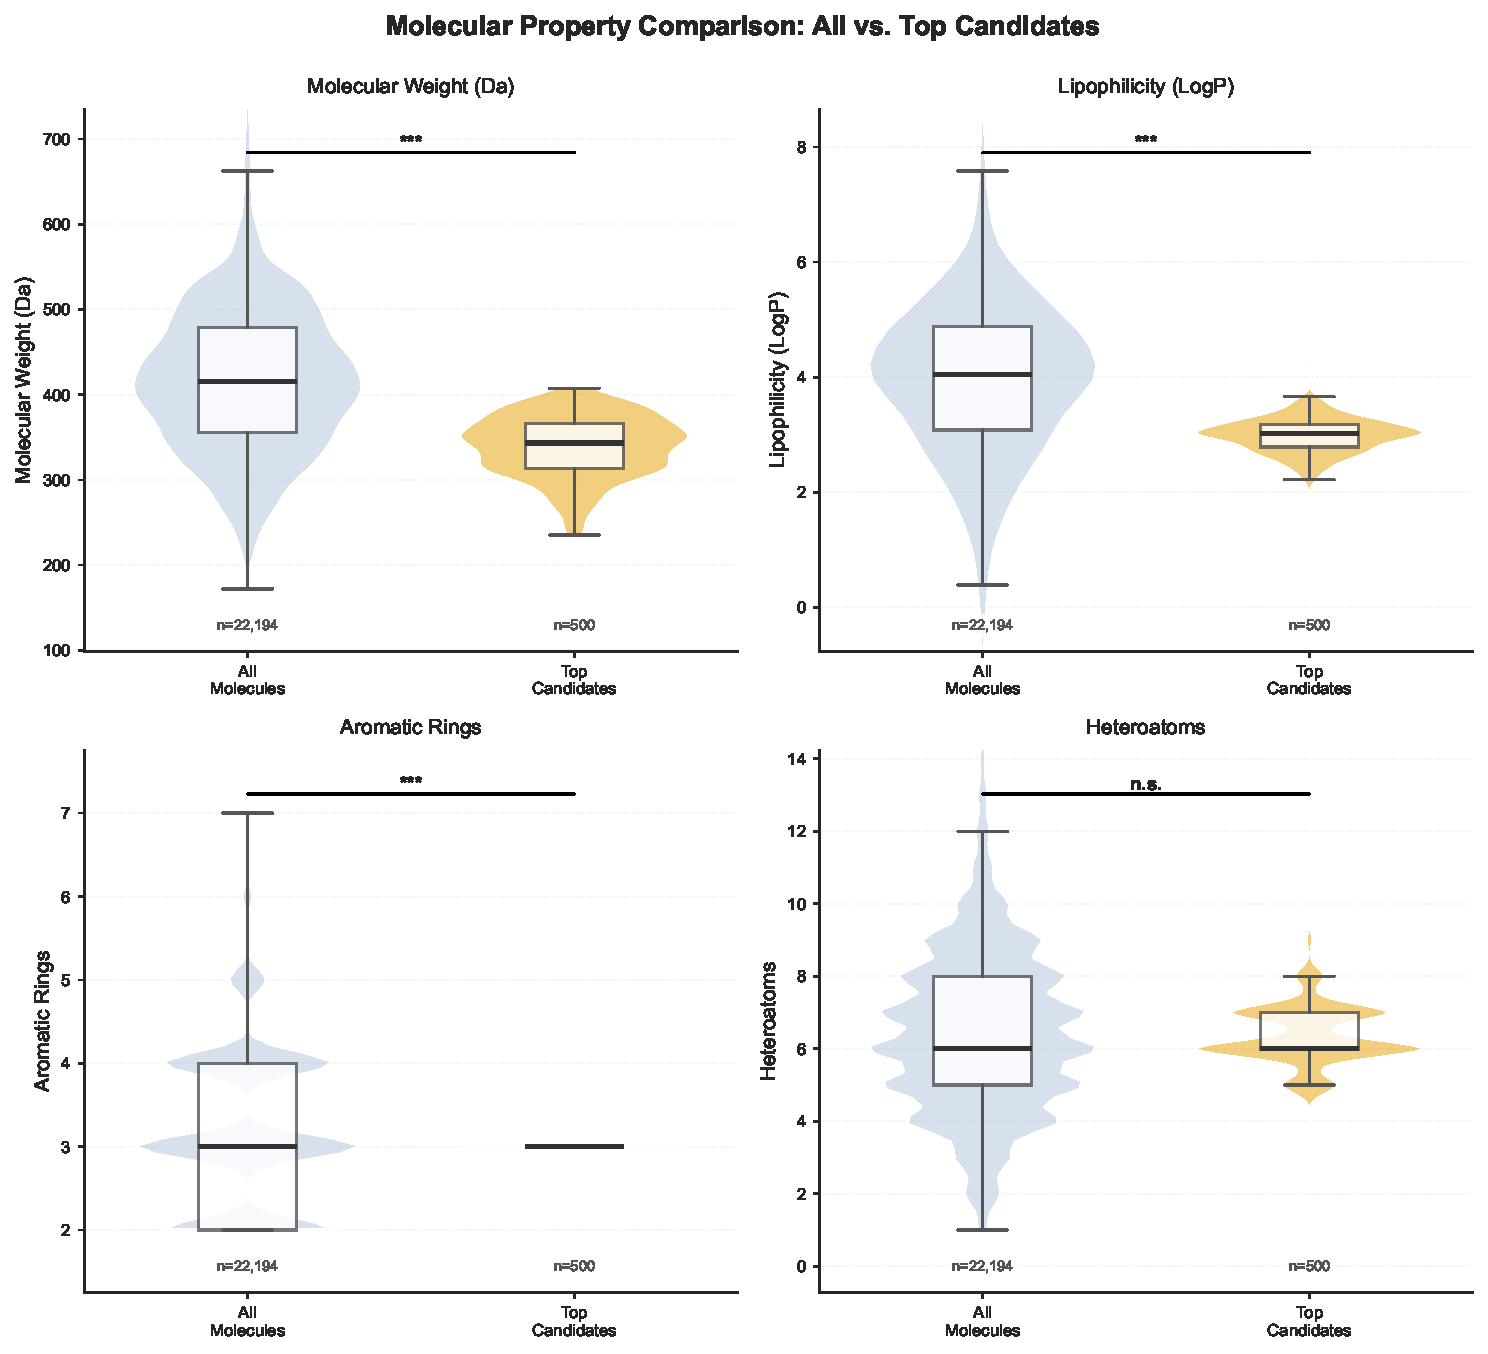
\includegraphics[width=0.75\textwidth]{figures/property_comparison.pdf}
  \caption{Property distributions of the enumerated library (\num{22194}
    fragment combinations, grey) versus the top \num{500} by heuristic TADF score
    (blue). Enrichment toward lower molecular weight reflects the scoring rule;
    these are unvalidated leads, not predicted emitters.}
  \label{fig:library_analysis}
\end{figure}

\subsection{Comparison with existing ML approaches}\label{subsec:comparison}

Before comparing models, we contextualise the absolute errors against three
baselines computed on the out-of-fold scaffold-CV predictions
(\cref{tab:baselines}; \qty{95}{\percent} bootstrap CIs, \num{2000} resamples):
the mean-value predictor (predicting $\bar{y}$ for every molecule,
MAE $= \qty{0.107}{\electronvolt}$), the median-value predictor
(MAE $= \qty{0.098}{\electronvolt}$), and a random-permutation null (mean MAE
over \num{1000} label shuffles, \qty{0.120}{\electronvolt}, \qty{95}{\percent}
interval \numrange{0.113}{0.127}).
The median is a tougher baseline than the mean because the experimental gap
distribution is right-skewed toward low-gap emitters; the permutation null is
clearly worse than either constant predictor, confirming that the trained model
exploits a real feature--label association rather than a fold artefact.
Our best model (RF--Morgan, MAE $= \qty{0.091}{\electronvolt}$) improves on the
mean baseline by \qty{15}{\percent}; the headline NTO model
(MAE $= \qty{0.096}{\electronvolt}$) improves by \qty{10.6}{\percent}
(\qty{0.011}{\electronvolt}, \qty{95}{\percent} CI on the paired difference
\numrange{0.003}{0.022}, excluding zero). The model edges even the skewed-median
baseline (\qty{0.098}{\electronvolt}).
This gain appears modest, but it must be interpreted against the
irreducible noise floor of the experimental corpus: the median inter-report
spread across the \num{102} multi-report molecules is
$\approx\qty{0.10}{\electronvolt}$, and for the worst-case molecule
$\qty{0.56}{\electronvolt}$ is observed.
An MAE of \qty{0.096}{\electronvolt} thus represents near-ceiling performance
given that noise floor, not near-zero improvement.
The excited-state step (NTO descriptors, MAE $= \qty{0.096}{\electronvolt}$)
offers no accuracy advantage over the purely structural approach, confirming
that label noise dominates over any feature advantage at the current scale
(\cref{subsec:limitations}).

\begin{table}[htbp]
  \centering
  \caption{Naive baselines versus the structure-based model on the same
    \num{231}-molecule out-of-fold scaffold-CV predictions. MAE in eV with
    \qty{95}{\percent} percentile-bootstrap CI (\num{2000} resamples); the
    permutation row is the mean and central \qty{95}{\percent} of \num{1000}
    label shuffles. The median outperforms the mean (right-skewed target); the
    permutation null is worse than both, so the model captures real signal.
    Values from \texttt{code/compute\_baselines.py}.}
  \label{tab:baselines}
  \begin{tabular}{lcc}
    \toprule
    Predictor & MAE (eV) & 95\% CI \\
    \midrule
    Mean predictor          & 0.107 & (0.092, 0.124) \\
    Median predictor        & 0.098 & (0.081, 0.118) \\
    Random-permutation null & 0.120 & (0.113, 0.127) \\
    \midrule
    NTO-RF (this work)      & \textbf{0.096} & (0.082, 0.109) \\
    \bottomrule
  \end{tabular}
\end{table}

Prior ML for TADF gaps is best read by the \emph{reference} it predicts, not by
the headline error alone (\cref{tab:prior_ml}). The low MAEs in the literature are
all against \emph{computed} targets: G\'omez-Bombarelli et
al.~\cite{Gomez-Bombarelli2016} trained a neural network to reproduce a TD-DFT gap
inside a $>$\num{e6}-molecule screen, Thapa et al.~\cite{Thapa2025} screened a
large virtual library against semi-empirically computed gaps, and Barneschi et al.~\cite{Barneschi2024}
reach \qty{0.02}{\electronvolt} with a 3D message-passing network---but against
ADC(2) values, and for inverted-gap molecules rather than donor--acceptor TADF.
Predicting the \emph{experimental} gap is the harder task this paper addresses:
Nigam et al.~\cite{Nigam2024} found direct regression of the measured gap so
unreliable that they fell back to a good/bad classifier. Our
\qty{0.096}{\electronvolt}, under scaffold cross-validation and with label and
reference noise accounted for, shows that cheap structural features nonetheless
track the experimental gap to within the $\approx\qty{0.1}{\electronvolt}$ floor
set by that noise. The contribution is not a record accuracy but a calibrated,
reproducible measure of how far cheap structural features reach, and a
demonstration that the excited-state step adds nothing to that task.

\begin{table*}[htbp]
  \centering
  \caption{Machine-learning prediction of TADF singlet--triplet gaps, ordered by
    reference type. Low MAEs are obtained only against \emph{computed} gaps;
    against the \emph{experimental} gap, errors are substantially larger and
    direct regression is sometimes abandoned. Only values reported in the
    cited sources are tabulated.}
  \label{tab:prior_ml}
  \small
  \begin{tabular}{lllll}
    \toprule
    Study & Model (features) & Set ($N$) & Reference & MAE (eV) \\
    \midrule
    G\'omez-Bombarelli 2016~\cite{Gomez-Bombarelli2016} & NN surrogate & $>$\num{e6} screened & TD-DFT (computed) & reproduces TD-DFT$^{a}$ \\
    Barneschi 2024~\cite{Barneschi2024} & 3D message-passing GNN & INVEST set & ADC(2) (computed) & 0.02$^{b}$ \\
    Nigam 2024~\cite{Nigam2024} & DNN classifier (Morgan FP) & GA-evolved & $\omega$B2PLYP$'$ (computed) & regression poor$^{c}$ \\
    \textbf{This work} & RF (NTO, structure) & 231 & experimental & \textbf{0.096} \\
    \bottomrule
  \end{tabular}

  \vspace{2pt}
  {\footnotesize\raggedright
   $^{a}$~Predicts the TD-DFT gap; no experimental-reference regression MAE reported.
   $^{b}$~Inverted-gap (Hund's-rule-violating) molecules, not donor--acceptor TADF.
   $^{c}$~Direct gap regression reported as poor; the deployed model is a good/bad
   classifier (\qtyrange{89}{98}{\percent} accuracy).\par}
\end{table*}

\subsection{Limitations}\label{subsec:limitations}

This study is bounded in several ways.
(1)~The experimental corpus is heterogeneous (mixed solvents and methods,
\qtyrange{0.1}{0.15}{\electronvolt} inter-report scatter); a single-source,
solvent-controlled dataset would be required to push below the present ceiling.
(2)~The model predicts a consensus gap, not solvatochromic or
conformer-dependent values.
(3)~We make no quantitative device claims. An earlier version of this work included
molecule-independent estimates for spin--orbit coupling, $k_\text{RISC}$, and
external quantum efficiency derived from literature medians. Following internal peer
review, these estimates were removed because the inter-molecular variance in these
quantities exceeds the precision of a scalar estimate by an order of magnitude. We
view this correction as an illustration of the iterative rigour appropriate to an
honest benchmark study: a median is not a molecule-specific prediction, and
reporting it as such would be misleading.
(4)~Ranking power is moderate ($\rho = 0.36$), so the model supports triage, not
final candidate selection.
(5)~The target is a single scalar, $\Delta E_\text{ST}(S_1\text{--}T_1)$. A small
$S_1$--$T_1$ gap is necessary but not sufficient for efficient delayed fluorescence:
the splitting of the triplet manifold ($T_1$--$T_2$) also governs reverse intersystem
crossing.\cite{Keruckiene2024} To gauge this we extracted $T_1$ and $T_2$ from the
CAM-B3LYP TD-DFT calculations for \num{14} emitters (\cref{SI-tab:manifold}): the
$T_1$--$T_2$ gap ranges \qtyrange{0.02}{1.50}{\electronvolt} and varies widely
\emph{among molecules with near-equal $\Delta E_\text{ST}$}, so a scalar-gap triage
cannot rank them on RISC propensity. This is, however, exactly the regime where the
excited-state pipeline earns its cost: the semi-empirical step is redundant for the
$S_1$--$T_1$ gap (\cref{subsec:nto_null}) but supplies the triplet-manifold information
that 2D structure cannot, a natural next target for the descriptors. Emitters with an
\emph{inverted} gap ($\Delta E_\text{ST} < 0$), which violate Hund's rule through
double-excitation character,\cite{Veglianti2025} are essentially unrepresented---only
\num{2} of \num{231} molecules carry a marginally negative reported gap, far too few to
characterise inverted-gap behaviour---so this emerging class is an explicit out-of-scope
future axis.
Future work targets a curated experimental benchmark and uncertainty-aware models
that report calibrated confidence alongside each prediction.
